\subsection{Geschichte}

Am 17.August 1982 wird erstmals eine CD der Öffentlichkeit vorgestellt. Die
ersten käuflichen Audio-CDs enthielten Chopins Walzer von Claudio Arrau und
\shorthandoff{"}"The Visitors"\shorthandon{"} von ABBA.

Die Entwicklung von Datenträgern mit einem laserbasiertem Auslesesystem beginnt
schon in den Siebziger Jahre. 1975 bringt Philips seinen ersten optischen
Datenträger auf den Markt, die Videodisc soll eine alternative zum
VHS-Videosystem darstellen, diese entwickelte sich aufgrund von geringen
Verkaufszahlen zu einem Flop.

\begin{figure}[h]
  \begin{center}
      \begin{minipage}[t]{0.3\textwidth}
        \begin{center}
            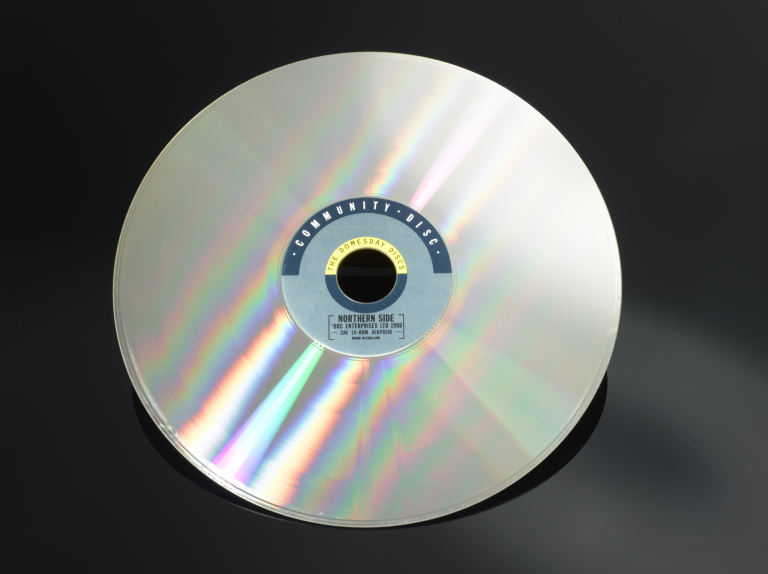
\includegraphics[height=0.1\textheight]{Bilder/Optische_Datentraeger_Die_Compact_Disc/Geschichte/videodisc.png}
            \caption[Laservision Videodisc \newline \url{http://www.sciencemuseum.org.uk/online_science/explore_our_collections/objects/index/smxg-8095649}]{Laservision Videodisc}
            \label{fig:videodisc}
        \end{center}
      \end{minipage}
      \hspace{0.025\textwidth}
      \begin{minipage}[t]{0.3\textwidth}
        \begin{center}
            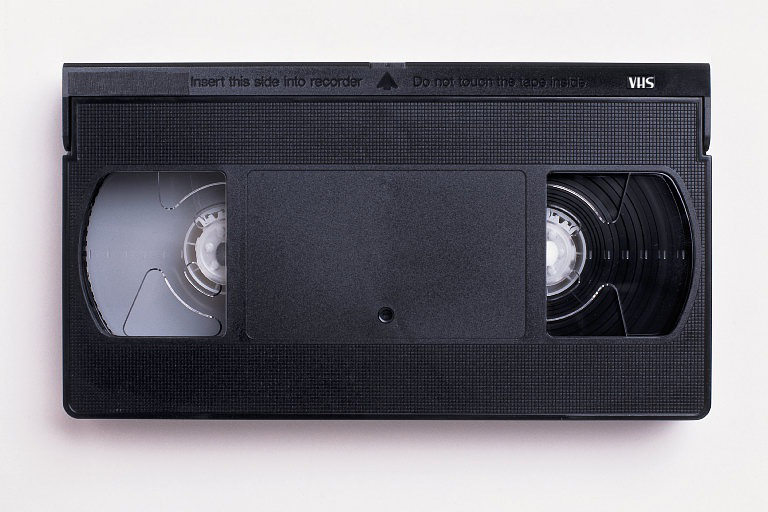
\includegraphics[height=0.1\textheight]{Bilder/Optische_Datentraeger_Die_Compact_Disc/Geschichte/vhs.png}
            \caption[VHS cassette \newline \url{https://upload.wikimedia.org/wikipedia/commons/6/67/VHS-cassette.jpg}]{VHS cassette}
            \label{fig:vhs}
        \end{center}
      \end{minipage}
  \end{center}
\end{figure}

Auf Basis der Videodisc entwickelt Philips bis 1977 die Compact Disc Digital
Audio. Sie besitzt einen Durchmesser von 11,5cm und eine Spielzeit von 60min.

Ab 1979 arbeiteten die beiden Musikgiganten Philips und Sony an einem
gemeinsamen CD-Standard. Man einigte sich auf einen Durchmesser von 12cm und
eine 75 minütige Spielzeit. Diese Standard ist bis heute von allen
CD-Herstellern anerkannt. \cite{cds}

Nach der Einigung auf einen gemeinsamen CD-Standard führten Sony und Philips
mehrere Verhandlungen mit Vertretern der großen Schallplattenproduzenten um sich
die Rechte an mehr Liedern für die CD zu sichern. Die Verhandlungen scheiterten
jedoch an der Skepsis der Verhandlungspartnern, da die Verkaufszahlen von
Schallplatten stark zurück gingen und die CD als potentieler Konkurrent für die
Schallplatte gesehen wird.

Nach den fehlgeschlagenen Verhandlungen beschlossen Philips und Sony sich
vorerst auf klassische Musik zu konzetrieren. Man vermutete hier einen
Kundenstamm, welcher eher bereit ist mehr Geld für eine bessere Klangqualität
auszugeben.

Der Durchbruch der CD gelang während den Salzburger Festspielen im April 1981.
Die beiden Konzerne konnten ein Publikum aus Musikkritikern von dem
Zukunftspotential der CD überzeugen. Die Begeisterung der Kritiker erfasste
ebenfalls die internationale Musikszene und bis März 1982 hatten acht
Schallplattenfirmen Verträge mit Philips und Sony unterschrieben. Die
Markteinführung geschieht am 17.August 1982. \cite{cuz}

Die CD verdrängte die Schallplatte innerhalb weniger Jahre fast komplett vom
Markt. Die \autoref{fig:umsatzcd} zeigt den Umsatz der deutschen Musikindustrie
mit dem jeweiligen Produkt. Der Umsatz durch die Vinylschallplatte, 1980 noch
das Umsatzstärkste Medium mit 760 Mio. Euro, sank bis 1987 erst allmählich und
bis 1992 rapide. Zu diesem Zeitpunkt betrug der Umsatz mit der CD ca. 1,7 Mrd.
Euro und rückte damit alle anderen Musikmedien in den Schatten. 1997 erreicht
die CD ihren Rekordumsatz mit 2,3 Mrd Euro. Ab 1997 sind die Verkaufszahlen
rückläufig aufgrund der Möglichkeit CDs als Privatperson zu
\shorthandoff{"}"brennen"\shorthandon{"} und dem zunehmenden legalen und
illegalen Angebot im Internet.

\begin{figure}[h]
  \begin{center}
      \begin{minipage}[t]{\textwidth}
        \begin{center}
            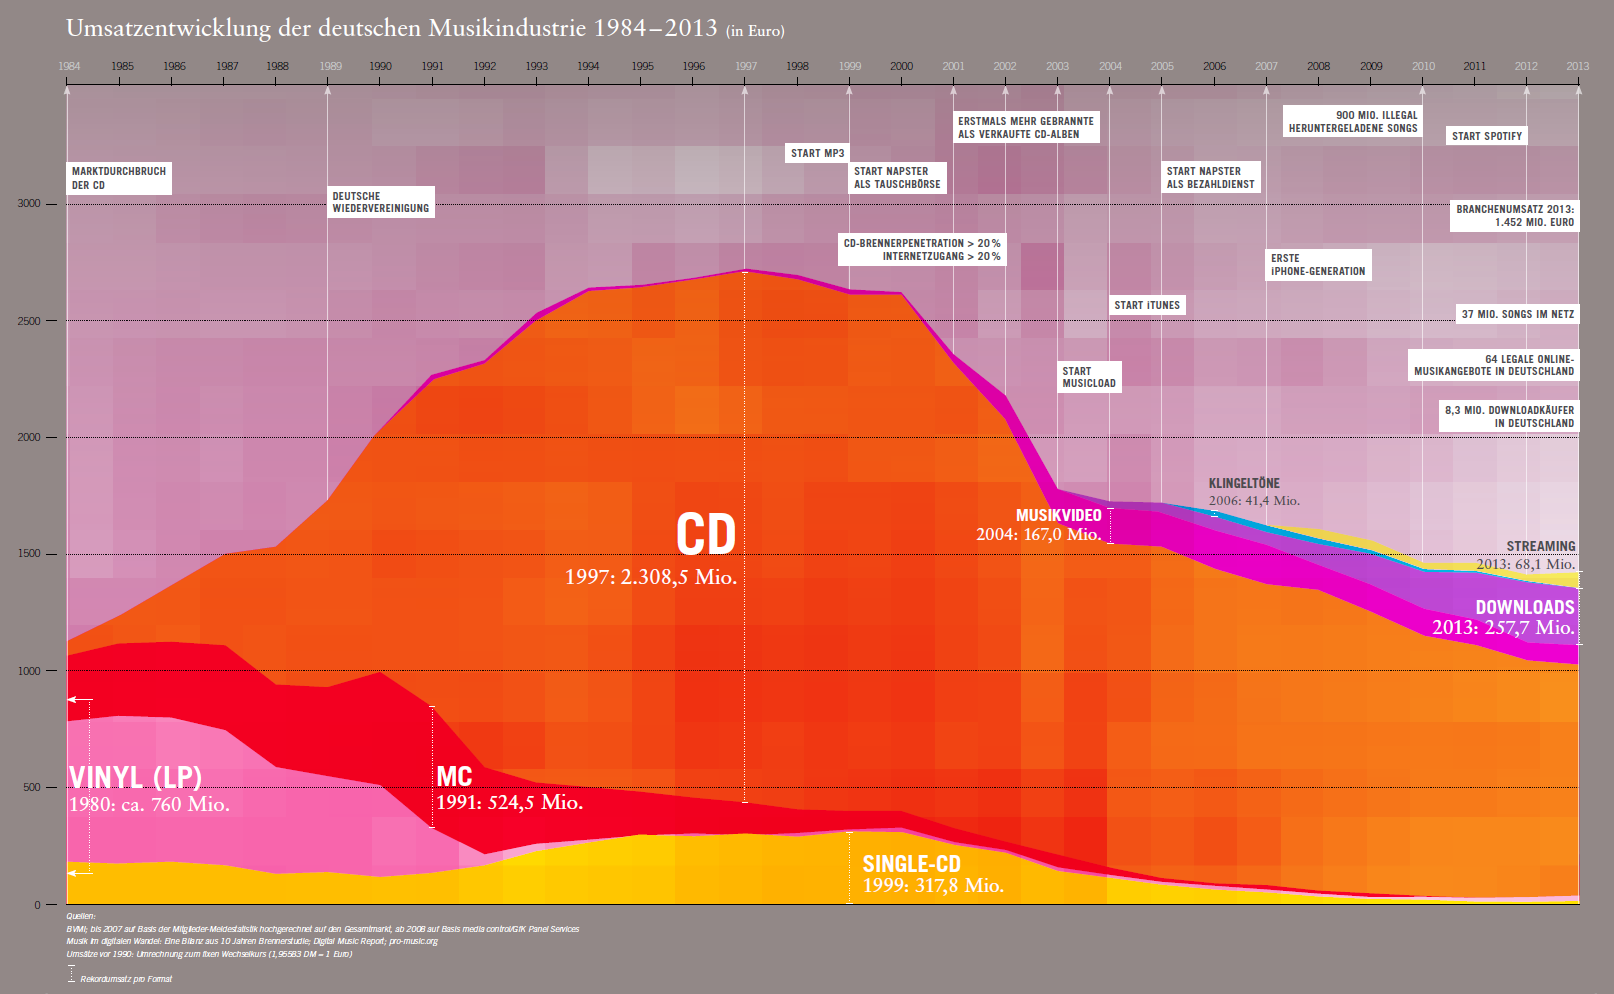
\includegraphics[width=\textwidth]{Bilder/Optische_Datentraeger_Die_Compact_Disc/Geschichte/umsatzcd.png}
            \caption[Umsatzentwicklung der deutschen Musikindustrie \newline \url{http://www.musikindustrie.de/uploads/media/140325\_BVMI\_2013\_Jahrbuch\_ePaper\_V02.pdf} S. 7 (zuletzt aufgerufen am 03.08.2015)]{Umsatzentwicklung der deutschen Musikindustrie}
            \label{fig:umsatzcd}
        \end{center}
      \end{minipage}
  \end{center}
\end{figure}

Trotz des damaligen relativ hohen Preise von ca. 40 Euro\footnote{unter
Berücksichtigung der Inflation} pro CD, überwiegen die folgenden Vorteile des
neuen Medium gegenüber der Schallplatte: \cite{cd1}

\begin{itemize*}
    \item keine Kratz- oder Knacktöne
    \item einfache Handhabung
    \item höhere Unempfindlichkeit gegenüber mechanischen Einwirkungen
    \item direkte Anwahl von Titeln
\end{itemize*}
